% Created by tikzDevice version 0.10.1 on 2017-12-03 20:41:03
% !TEX encoding = UTF-8 Unicode
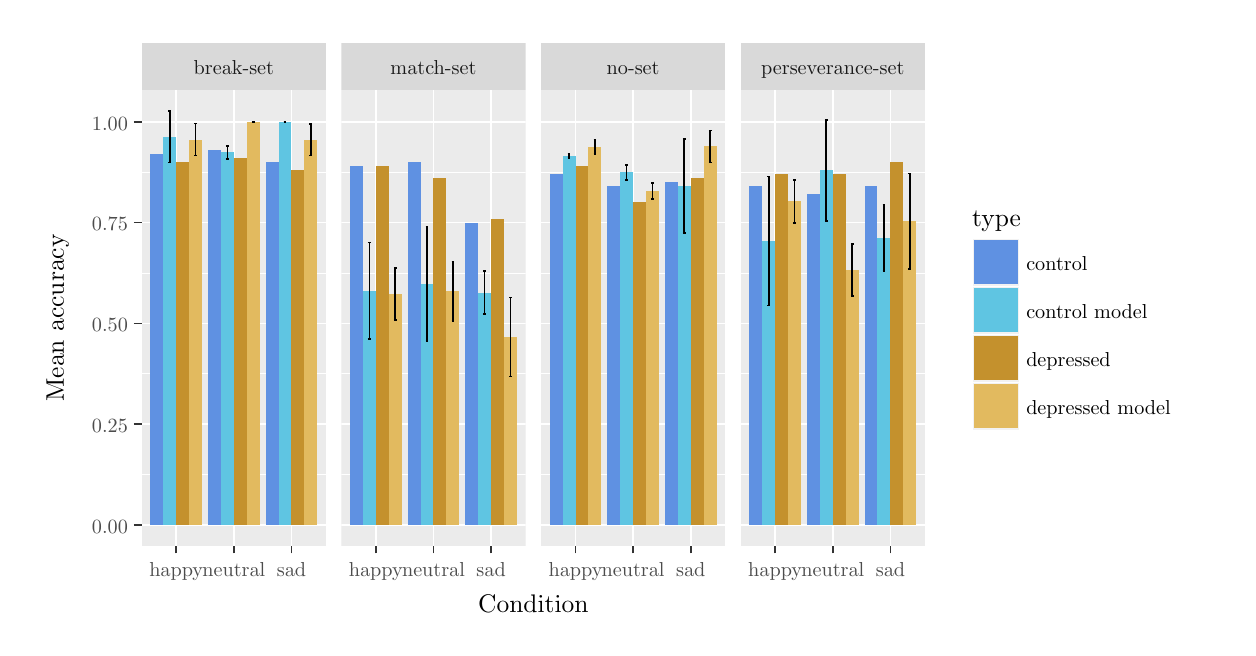
\begin{tikzpicture}[x=1pt,y=1pt]
\definecolor{fillColor}{RGB}{255,255,255}
\path[use as bounding box,fill=fillColor,fill opacity=0.00] (0,0) rectangle (433.62,216.81);
\begin{scope}
\path[clip] (  0.00,  0.00) rectangle (433.62,216.81);
\definecolor{drawColor}{RGB}{255,255,255}
\definecolor{fillColor}{RGB}{255,255,255}

\path[draw=drawColor,line width= 0.6pt,line join=round,line cap=round,fill=fillColor] (  0.00,  0.00) rectangle (433.62,216.81);
\end{scope}
\begin{scope}
\path[clip] ( 41.17, 29.59) rectangle (107.82,194.25);
\definecolor{fillColor}{gray}{0.92}

\path[fill=fillColor] ( 41.17, 29.59) rectangle (107.82,194.25);
\definecolor{drawColor}{RGB}{255,255,255}

\path[draw=drawColor,line width= 0.3pt,line join=round] ( 41.17, 55.29) --
	(107.82, 55.29);

\path[draw=drawColor,line width= 0.3pt,line join=round] ( 41.17, 91.72) --
	(107.82, 91.72);

\path[draw=drawColor,line width= 0.3pt,line join=round] ( 41.17,128.16) --
	(107.82,128.16);

\path[draw=drawColor,line width= 0.3pt,line join=round] ( 41.17,164.60) --
	(107.82,164.60);

\path[draw=drawColor,line width= 0.6pt,line join=round] ( 41.17, 37.07) --
	(107.82, 37.07);

\path[draw=drawColor,line width= 0.6pt,line join=round] ( 41.17, 73.51) --
	(107.82, 73.51);

\path[draw=drawColor,line width= 0.6pt,line join=round] ( 41.17,109.94) --
	(107.82,109.94);

\path[draw=drawColor,line width= 0.6pt,line join=round] ( 41.17,146.38) --
	(107.82,146.38);

\path[draw=drawColor,line width= 0.6pt,line join=round] ( 41.17,182.81) --
	(107.82,182.81);

\path[draw=drawColor,line width= 0.6pt,line join=round] ( 53.67, 29.59) --
	( 53.67,194.25);

\path[draw=drawColor,line width= 0.6pt,line join=round] ( 74.50, 29.59) --
	( 74.50,194.25);

\path[draw=drawColor,line width= 0.6pt,line join=round] ( 95.32, 29.59) --
	( 95.32,194.25);
\definecolor{fillColor}{RGB}{226,186,95}

\path[fill=fillColor] ( 58.36, 37.07) rectangle ( 63.04,176.38);
\definecolor{fillColor}{RGB}{196,145,45}

\path[fill=fillColor] ( 53.67, 37.07) rectangle ( 58.36,168.24);
\definecolor{fillColor}{RGB}{95,197,226}

\path[fill=fillColor] ( 48.98, 37.07) rectangle ( 53.67,177.42);
\definecolor{fillColor}{RGB}{95,145,226}

\path[fill=fillColor] ( 44.30, 37.07) rectangle ( 48.98,171.15);
\definecolor{fillColor}{RGB}{226,186,95}

\path[fill=fillColor] ( 79.18, 37.07) rectangle ( 83.87,182.81);
\definecolor{fillColor}{RGB}{196,145,45}

\path[fill=fillColor] ( 74.50, 37.07) rectangle ( 79.18,169.70);
\definecolor{fillColor}{RGB}{95,197,226}

\path[fill=fillColor] ( 69.81, 37.07) rectangle ( 74.50,171.80);
\definecolor{fillColor}{RGB}{95,145,226}

\path[fill=fillColor] ( 65.12, 37.07) rectangle ( 69.81,172.61);
\definecolor{fillColor}{RGB}{226,186,95}

\path[fill=fillColor] (100.01, 37.07) rectangle (104.69,176.31);
\definecolor{fillColor}{RGB}{196,145,45}

\path[fill=fillColor] ( 95.32, 37.07) rectangle (100.01,165.32);
\definecolor{fillColor}{RGB}{95,197,226}

\path[fill=fillColor] ( 90.64, 37.07) rectangle ( 95.32,182.81);
\definecolor{fillColor}{RGB}{95,145,226}

\path[fill=fillColor] ( 85.95, 37.07) rectangle ( 90.64,168.24);
\definecolor{drawColor}{RGB}{0,0,0}

\path[draw=drawColor,line width= 0.6pt,line join=round] ( 60.18,182.16) --
	( 61.22,182.16);

\path[draw=drawColor,line width= 0.6pt,line join=round] ( 60.70,182.16) --
	( 60.70,170.59);

\path[draw=drawColor,line width= 0.6pt,line join=round] ( 60.18,170.59) --
	( 61.22,170.59);

\path[draw=drawColor,line width= 0.6pt,line join=round] ( 50.81,186.76) --
	( 51.85,186.76);

\path[draw=drawColor,line width= 0.6pt,line join=round] ( 51.33,186.76) --
	( 51.33,168.07);

\path[draw=drawColor,line width= 0.6pt,line join=round] ( 50.81,168.07) --
	( 51.85,168.07);

\path[draw=drawColor,line width= 0.6pt,line join=round] ( 81.00,182.81) --
	( 82.05,182.81);

\path[draw=drawColor,line width= 0.6pt,line join=round] ( 81.52,182.81) --
	( 81.52,182.81);

\path[draw=drawColor,line width= 0.6pt,line join=round] ( 81.00,182.81) --
	( 82.05,182.81);

\path[draw=drawColor,line width= 0.6pt,line join=round] ( 71.63,174.15) --
	( 72.67,174.15);

\path[draw=drawColor,line width= 0.6pt,line join=round] ( 72.15,174.15) --
	( 72.15,169.46);

\path[draw=drawColor,line width= 0.6pt,line join=round] ( 71.63,169.46) --
	( 72.67,169.46);

\path[draw=drawColor,line width= 0.6pt,line join=round] (101.83,181.98) --
	(102.87,181.98);

\path[draw=drawColor,line width= 0.6pt,line join=round] (102.35,181.98) --
	(102.35,170.63);

\path[draw=drawColor,line width= 0.6pt,line join=round] (101.83,170.63) --
	(102.87,170.63);

\path[draw=drawColor,line width= 0.6pt,line join=round] ( 92.46,182.81) --
	( 93.50,182.81);

\path[draw=drawColor,line width= 0.6pt,line join=round] ( 92.98,182.81) --
	( 92.98,182.81);

\path[draw=drawColor,line width= 0.6pt,line join=round] ( 92.46,182.81) --
	( 93.50,182.81);
\end{scope}
\begin{scope}
\path[clip] (113.32, 29.59) rectangle (179.96,194.25);
\definecolor{fillColor}{gray}{0.92}

\path[fill=fillColor] (113.32, 29.59) rectangle (179.96,194.25);
\definecolor{drawColor}{RGB}{255,255,255}

\path[draw=drawColor,line width= 0.3pt,line join=round] (113.32, 55.29) --
	(179.96, 55.29);

\path[draw=drawColor,line width= 0.3pt,line join=round] (113.32, 91.72) --
	(179.96, 91.72);

\path[draw=drawColor,line width= 0.3pt,line join=round] (113.32,128.16) --
	(179.96,128.16);

\path[draw=drawColor,line width= 0.3pt,line join=round] (113.32,164.60) --
	(179.96,164.60);

\path[draw=drawColor,line width= 0.6pt,line join=round] (113.32, 37.07) --
	(179.96, 37.07);

\path[draw=drawColor,line width= 0.6pt,line join=round] (113.32, 73.51) --
	(179.96, 73.51);

\path[draw=drawColor,line width= 0.6pt,line join=round] (113.32,109.94) --
	(179.96,109.94);

\path[draw=drawColor,line width= 0.6pt,line join=round] (113.32,146.38) --
	(179.96,146.38);

\path[draw=drawColor,line width= 0.6pt,line join=round] (113.32,182.81) --
	(179.96,182.81);

\path[draw=drawColor,line width= 0.6pt,line join=round] (125.81, 29.59) --
	(125.81,194.25);

\path[draw=drawColor,line width= 0.6pt,line join=round] (146.64, 29.59) --
	(146.64,194.25);

\path[draw=drawColor,line width= 0.6pt,line join=round] (167.47, 29.59) --
	(167.47,194.25);
\definecolor{fillColor}{RGB}{226,186,95}

\path[fill=fillColor] (130.50, 37.07) rectangle (135.19,120.66);
\definecolor{fillColor}{RGB}{196,145,45}

\path[fill=fillColor] (125.81, 37.07) rectangle (130.50,166.78);
\definecolor{fillColor}{RGB}{95,197,226}

\path[fill=fillColor] (121.13, 37.07) rectangle (125.81,121.75);
\definecolor{fillColor}{RGB}{95,145,226}

\path[fill=fillColor] (116.44, 37.07) rectangle (121.13,166.78);
\definecolor{fillColor}{RGB}{226,186,95}

\path[fill=fillColor] (151.33, 37.07) rectangle (156.01,121.49);
\definecolor{fillColor}{RGB}{196,145,45}

\path[fill=fillColor] (146.64, 37.07) rectangle (151.33,162.41);
\definecolor{fillColor}{RGB}{95,197,226}

\path[fill=fillColor] (141.95, 37.07) rectangle (146.64,124.24);
\definecolor{fillColor}{RGB}{95,145,226}

\path[fill=fillColor] (137.27, 37.07) rectangle (141.95,168.24);
\definecolor{fillColor}{RGB}{226,186,95}

\path[fill=fillColor] (172.15, 37.07) rectangle (176.84,105.07);
\definecolor{fillColor}{RGB}{196,145,45}

\path[fill=fillColor] (167.47, 37.07) rectangle (172.15,147.84);
\definecolor{fillColor}{RGB}{95,197,226}

\path[fill=fillColor] (162.78, 37.07) rectangle (167.47,121.07);
\definecolor{fillColor}{RGB}{95,145,226}

\path[fill=fillColor] (158.10, 37.07) rectangle (162.78,146.38);
\definecolor{drawColor}{RGB}{0,0,0}

\path[draw=drawColor,line width= 0.6pt,line join=round] (132.32,130.06) --
	(133.36,130.06);

\path[draw=drawColor,line width= 0.6pt,line join=round] (132.84,130.06) --
	(132.84,111.27);

\path[draw=drawColor,line width= 0.6pt,line join=round] (132.32,111.27) --
	(133.36,111.27);

\path[draw=drawColor,line width= 0.6pt,line join=round] (122.95,139.21) --
	(123.99,139.21);

\path[draw=drawColor,line width= 0.6pt,line join=round] (123.47,139.21) --
	(123.47,104.28);

\path[draw=drawColor,line width= 0.6pt,line join=round] (122.95,104.28) --
	(123.99,104.28);

\path[draw=drawColor,line width= 0.6pt,line join=round] (153.15,132.20) --
	(154.19,132.20);

\path[draw=drawColor,line width= 0.6pt,line join=round] (153.67,132.20) --
	(153.67,110.78);

\path[draw=drawColor,line width= 0.6pt,line join=round] (153.15,110.78) --
	(154.19,110.78);

\path[draw=drawColor,line width= 0.6pt,line join=round] (143.78,144.91) --
	(144.82,144.91);

\path[draw=drawColor,line width= 0.6pt,line join=round] (144.30,144.91) --
	(144.30,103.56);

\path[draw=drawColor,line width= 0.6pt,line join=round] (143.78,103.56) --
	(144.82,103.56);

\path[draw=drawColor,line width= 0.6pt,line join=round] (173.98,119.35) --
	(175.02,119.35);

\path[draw=drawColor,line width= 0.6pt,line join=round] (174.50,119.35) --
	(174.50, 90.79);

\path[draw=drawColor,line width= 0.6pt,line join=round] (173.98, 90.79) --
	(175.02, 90.79);

\path[draw=drawColor,line width= 0.6pt,line join=round] (164.60,128.84) --
	(165.64,128.84);

\path[draw=drawColor,line width= 0.6pt,line join=round] (165.12,128.84) --
	(165.12,113.30);

\path[draw=drawColor,line width= 0.6pt,line join=round] (164.60,113.30) --
	(165.64,113.30);
\end{scope}
\begin{scope}
\path[clip] (185.46, 29.59) rectangle (252.11,194.25);
\definecolor{fillColor}{gray}{0.92}

\path[fill=fillColor] (185.46, 29.59) rectangle (252.11,194.25);
\definecolor{drawColor}{RGB}{255,255,255}

\path[draw=drawColor,line width= 0.3pt,line join=round] (185.46, 55.29) --
	(252.11, 55.29);

\path[draw=drawColor,line width= 0.3pt,line join=round] (185.46, 91.72) --
	(252.11, 91.72);

\path[draw=drawColor,line width= 0.3pt,line join=round] (185.46,128.16) --
	(252.11,128.16);

\path[draw=drawColor,line width= 0.3pt,line join=round] (185.46,164.60) --
	(252.11,164.60);

\path[draw=drawColor,line width= 0.6pt,line join=round] (185.46, 37.07) --
	(252.11, 37.07);

\path[draw=drawColor,line width= 0.6pt,line join=round] (185.46, 73.51) --
	(252.11, 73.51);

\path[draw=drawColor,line width= 0.6pt,line join=round] (185.46,109.94) --
	(252.11,109.94);

\path[draw=drawColor,line width= 0.6pt,line join=round] (185.46,146.38) --
	(252.11,146.38);

\path[draw=drawColor,line width= 0.6pt,line join=round] (185.46,182.81) --
	(252.11,182.81);

\path[draw=drawColor,line width= 0.6pt,line join=round] (197.96, 29.59) --
	(197.96,194.25);

\path[draw=drawColor,line width= 0.6pt,line join=round] (218.79, 29.59) --
	(218.79,194.25);

\path[draw=drawColor,line width= 0.6pt,line join=round] (239.61, 29.59) --
	(239.61,194.25);
\definecolor{fillColor}{RGB}{226,186,95}

\path[fill=fillColor] (202.64, 37.07) rectangle (207.33,173.74);
\definecolor{fillColor}{RGB}{196,145,45}

\path[fill=fillColor] (197.96, 37.07) rectangle (202.64,166.78);
\definecolor{fillColor}{RGB}{95,197,226}

\path[fill=fillColor] (193.27, 37.07) rectangle (197.96,170.53);
\definecolor{fillColor}{RGB}{95,145,226}

\path[fill=fillColor] (188.59, 37.07) rectangle (193.27,163.87);
\definecolor{fillColor}{RGB}{226,186,95}

\path[fill=fillColor] (223.47, 37.07) rectangle (228.16,157.76);
\definecolor{fillColor}{RGB}{196,145,45}

\path[fill=fillColor] (218.79, 37.07) rectangle (223.47,153.66);
\definecolor{fillColor}{RGB}{95,197,226}

\path[fill=fillColor] (214.10, 37.07) rectangle (218.79,164.53);
\definecolor{fillColor}{RGB}{95,145,226}

\path[fill=fillColor] (209.41, 37.07) rectangle (214.10,159.49);
\definecolor{fillColor}{RGB}{226,186,95}

\path[fill=fillColor] (244.30, 37.07) rectangle (248.98,173.87);
\definecolor{fillColor}{RGB}{196,145,45}

\path[fill=fillColor] (239.61, 37.07) rectangle (244.30,162.41);
\definecolor{fillColor}{RGB}{95,197,226}

\path[fill=fillColor] (234.93, 37.07) rectangle (239.61,159.50);
\definecolor{fillColor}{RGB}{95,145,226}

\path[fill=fillColor] (230.24, 37.07) rectangle (234.93,160.95);
\definecolor{drawColor}{RGB}{0,0,0}

\path[draw=drawColor,line width= 0.6pt,line join=round] (204.47,176.26) --
	(205.51,176.26);

\path[draw=drawColor,line width= 0.6pt,line join=round] (204.99,176.26) --
	(204.99,171.22);

\path[draw=drawColor,line width= 0.6pt,line join=round] (204.47,171.22) --
	(205.51,171.22);

\path[draw=drawColor,line width= 0.6pt,line join=round] (195.10,171.23) --
	(196.14,171.23);

\path[draw=drawColor,line width= 0.6pt,line join=round] (195.62,171.23) --
	(195.62,169.83);

\path[draw=drawColor,line width= 0.6pt,line join=round] (195.10,169.83) --
	(196.14,169.83);

\path[draw=drawColor,line width= 0.6pt,line join=round] (225.29,160.61) --
	(226.34,160.61);

\path[draw=drawColor,line width= 0.6pt,line join=round] (225.81,160.61) --
	(225.81,154.91);

\path[draw=drawColor,line width= 0.6pt,line join=round] (225.29,154.91) --
	(226.34,154.91);

\path[draw=drawColor,line width= 0.6pt,line join=round] (215.92,167.29) --
	(216.96,167.29);

\path[draw=drawColor,line width= 0.6pt,line join=round] (216.44,167.29) --
	(216.44,161.77);

\path[draw=drawColor,line width= 0.6pt,line join=round] (215.92,161.77) --
	(216.96,161.77);

\path[draw=drawColor,line width= 0.6pt,line join=round] (246.12,179.64) --
	(247.16,179.64);

\path[draw=drawColor,line width= 0.6pt,line join=round] (246.64,179.64) --
	(246.64,168.11);

\path[draw=drawColor,line width= 0.6pt,line join=round] (246.12,168.11) --
	(247.16,168.11);

\path[draw=drawColor,line width= 0.6pt,line join=round] (236.75,176.47) --
	(237.79,176.47);

\path[draw=drawColor,line width= 0.6pt,line join=round] (237.27,176.47) --
	(237.27,142.54);

\path[draw=drawColor,line width= 0.6pt,line join=round] (236.75,142.54) --
	(237.79,142.54);
\end{scope}
\begin{scope}
\path[clip] (257.61, 29.59) rectangle (324.25,194.25);
\definecolor{fillColor}{gray}{0.92}

\path[fill=fillColor] (257.61, 29.59) rectangle (324.25,194.25);
\definecolor{drawColor}{RGB}{255,255,255}

\path[draw=drawColor,line width= 0.3pt,line join=round] (257.61, 55.29) --
	(324.25, 55.29);

\path[draw=drawColor,line width= 0.3pt,line join=round] (257.61, 91.72) --
	(324.25, 91.72);

\path[draw=drawColor,line width= 0.3pt,line join=round] (257.61,128.16) --
	(324.25,128.16);

\path[draw=drawColor,line width= 0.3pt,line join=round] (257.61,164.60) --
	(324.25,164.60);

\path[draw=drawColor,line width= 0.6pt,line join=round] (257.61, 37.07) --
	(324.25, 37.07);

\path[draw=drawColor,line width= 0.6pt,line join=round] (257.61, 73.51) --
	(324.25, 73.51);

\path[draw=drawColor,line width= 0.6pt,line join=round] (257.61,109.94) --
	(324.25,109.94);

\path[draw=drawColor,line width= 0.6pt,line join=round] (257.61,146.38) --
	(324.25,146.38);

\path[draw=drawColor,line width= 0.6pt,line join=round] (257.61,182.81) --
	(324.25,182.81);

\path[draw=drawColor,line width= 0.6pt,line join=round] (270.10, 29.59) --
	(270.10,194.25);

\path[draw=drawColor,line width= 0.6pt,line join=round] (290.93, 29.59) --
	(290.93,194.25);

\path[draw=drawColor,line width= 0.6pt,line join=round] (311.76, 29.59) --
	(311.76,194.25);
\definecolor{fillColor}{RGB}{226,186,95}

\path[fill=fillColor] (274.79, 37.07) rectangle (279.48,154.01);
\definecolor{fillColor}{RGB}{196,145,45}

\path[fill=fillColor] (270.10, 37.07) rectangle (274.79,163.87);
\definecolor{fillColor}{RGB}{95,197,226}

\path[fill=fillColor] (265.42, 37.07) rectangle (270.10,139.77);
\definecolor{fillColor}{RGB}{95,145,226}

\path[fill=fillColor] (260.73, 37.07) rectangle (265.42,159.49);
\definecolor{fillColor}{RGB}{226,186,95}

\path[fill=fillColor] (295.62, 37.07) rectangle (300.30,129.20);
\definecolor{fillColor}{RGB}{196,145,45}

\path[fill=fillColor] (290.93, 37.07) rectangle (295.62,163.87);
\definecolor{fillColor}{RGB}{95,197,226}

\path[fill=fillColor] (286.24, 37.07) rectangle (290.93,165.27);
\definecolor{fillColor}{RGB}{95,145,226}

\path[fill=fillColor] (281.56, 37.07) rectangle (286.24,156.58);
\definecolor{fillColor}{RGB}{226,186,95}

\path[fill=fillColor] (316.44, 37.07) rectangle (321.13,146.86);
\definecolor{fillColor}{RGB}{196,145,45}

\path[fill=fillColor] (311.76, 37.07) rectangle (316.44,168.24);
\definecolor{fillColor}{RGB}{95,197,226}

\path[fill=fillColor] (307.07, 37.07) rectangle (311.76,140.86);
\definecolor{fillColor}{RGB}{95,145,226}

\path[fill=fillColor] (302.39, 37.07) rectangle (307.07,159.49);
\definecolor{drawColor}{RGB}{0,0,0}

\path[draw=drawColor,line width= 0.6pt,line join=round] (276.61,161.83) --
	(277.65,161.83);

\path[draw=drawColor,line width= 0.6pt,line join=round] (277.13,161.83) --
	(277.13,146.20);

\path[draw=drawColor,line width= 0.6pt,line join=round] (276.61,146.20) --
	(277.65,146.20);

\path[draw=drawColor,line width= 0.6pt,line join=round] (267.24,163.09) --
	(268.28,163.09);

\path[draw=drawColor,line width= 0.6pt,line join=round] (267.76,163.09) --
	(267.76,116.44);

\path[draw=drawColor,line width= 0.6pt,line join=round] (267.24,116.44) --
	(268.28,116.44);

\path[draw=drawColor,line width= 0.6pt,line join=round] (297.44,138.61) --
	(298.48,138.61);

\path[draw=drawColor,line width= 0.6pt,line join=round] (297.96,138.61) --
	(297.96,119.79);

\path[draw=drawColor,line width= 0.6pt,line join=round] (297.44,119.79) --
	(298.48,119.79);

\path[draw=drawColor,line width= 0.6pt,line join=round] (288.07,183.53) --
	(289.11,183.53);

\path[draw=drawColor,line width= 0.6pt,line join=round] (288.59,183.53) --
	(288.59,147.02);

\path[draw=drawColor,line width= 0.6pt,line join=round] (288.07,147.02) --
	(289.11,147.02);

\path[draw=drawColor,line width= 0.6pt,line join=round] (318.27,164.06) --
	(319.31,164.06);

\path[draw=drawColor,line width= 0.6pt,line join=round] (318.79,164.06) --
	(318.79,129.66);

\path[draw=drawColor,line width= 0.6pt,line join=round] (318.27,129.66) --
	(319.31,129.66);

\path[draw=drawColor,line width= 0.6pt,line join=round] (308.89,152.88) --
	(309.93,152.88);

\path[draw=drawColor,line width= 0.6pt,line join=round] (309.41,152.88) --
	(309.41,128.84);

\path[draw=drawColor,line width= 0.6pt,line join=round] (308.89,128.84) --
	(309.93,128.84);
\end{scope}
\begin{scope}
\path[clip] ( 41.17,194.25) rectangle (107.82,211.31);
\definecolor{fillColor}{gray}{0.85}

\path[fill=fillColor] ( 41.17,194.25) rectangle (107.82,211.31);
\definecolor{drawColor}{gray}{0.10}

\node[text=drawColor,anchor=base,inner sep=0pt, outer sep=0pt, scale=  0.73] at ( 74.50,199.75) {break-set};
\end{scope}
\begin{scope}
\path[clip] (113.32,194.25) rectangle (179.96,211.31);
\definecolor{fillColor}{gray}{0.85}

\path[fill=fillColor] (113.32,194.25) rectangle (179.96,211.31);
\definecolor{drawColor}{gray}{0.10}

\node[text=drawColor,anchor=base,inner sep=0pt, outer sep=0pt, scale=  0.73] at (146.64,199.75) {match-set};
\end{scope}
\begin{scope}
\path[clip] (185.46,194.25) rectangle (252.11,211.31);
\definecolor{fillColor}{gray}{0.85}

\path[fill=fillColor] (185.46,194.25) rectangle (252.11,211.31);
\definecolor{drawColor}{gray}{0.10}

\node[text=drawColor,anchor=base,inner sep=0pt, outer sep=0pt, scale=  0.73] at (218.79,199.75) {no-set};
\end{scope}
\begin{scope}
\path[clip] (257.61,194.25) rectangle (324.25,211.31);
\definecolor{fillColor}{gray}{0.85}

\path[fill=fillColor] (257.61,194.25) rectangle (324.25,211.31);
\definecolor{drawColor}{gray}{0.10}

\node[text=drawColor,anchor=base,inner sep=0pt, outer sep=0pt, scale=  0.73] at (290.93,199.75) {perseverance-set};
\end{scope}
\begin{scope}
\path[clip] (  0.00,  0.00) rectangle (433.62,216.81);
\definecolor{drawColor}{gray}{0.20}

\path[draw=drawColor,line width= 0.6pt,line join=round] ( 53.67, 26.84) --
	( 53.67, 29.59);

\path[draw=drawColor,line width= 0.6pt,line join=round] ( 74.50, 26.84) --
	( 74.50, 29.59);

\path[draw=drawColor,line width= 0.6pt,line join=round] ( 95.32, 26.84) --
	( 95.32, 29.59);
\end{scope}
\begin{scope}
\path[clip] (  0.00,  0.00) rectangle (433.62,216.81);
\definecolor{drawColor}{gray}{0.30}

\node[text=drawColor,anchor=base,inner sep=0pt, outer sep=0pt, scale=  0.73] at ( 53.67, 18.58) {happy};

\node[text=drawColor,anchor=base,inner sep=0pt, outer sep=0pt, scale=  0.73] at ( 74.50, 18.58) {neutral};

\node[text=drawColor,anchor=base,inner sep=0pt, outer sep=0pt, scale=  0.73] at ( 95.32, 18.58) {sad};
\end{scope}
\begin{scope}
\path[clip] (  0.00,  0.00) rectangle (433.62,216.81);
\definecolor{drawColor}{gray}{0.20}

\path[draw=drawColor,line width= 0.6pt,line join=round] (125.81, 26.84) --
	(125.81, 29.59);

\path[draw=drawColor,line width= 0.6pt,line join=round] (146.64, 26.84) --
	(146.64, 29.59);

\path[draw=drawColor,line width= 0.6pt,line join=round] (167.47, 26.84) --
	(167.47, 29.59);
\end{scope}
\begin{scope}
\path[clip] (  0.00,  0.00) rectangle (433.62,216.81);
\definecolor{drawColor}{gray}{0.30}

\node[text=drawColor,anchor=base,inner sep=0pt, outer sep=0pt, scale=  0.73] at (125.81, 18.58) {happy};

\node[text=drawColor,anchor=base,inner sep=0pt, outer sep=0pt, scale=  0.73] at (146.64, 18.58) {neutral};

\node[text=drawColor,anchor=base,inner sep=0pt, outer sep=0pt, scale=  0.73] at (167.47, 18.58) {sad};
\end{scope}
\begin{scope}
\path[clip] (  0.00,  0.00) rectangle (433.62,216.81);
\definecolor{drawColor}{gray}{0.20}

\path[draw=drawColor,line width= 0.6pt,line join=round] (197.96, 26.84) --
	(197.96, 29.59);

\path[draw=drawColor,line width= 0.6pt,line join=round] (218.79, 26.84) --
	(218.79, 29.59);

\path[draw=drawColor,line width= 0.6pt,line join=round] (239.61, 26.84) --
	(239.61, 29.59);
\end{scope}
\begin{scope}
\path[clip] (  0.00,  0.00) rectangle (433.62,216.81);
\definecolor{drawColor}{gray}{0.30}

\node[text=drawColor,anchor=base,inner sep=0pt, outer sep=0pt, scale=  0.73] at (197.96, 18.58) {happy};

\node[text=drawColor,anchor=base,inner sep=0pt, outer sep=0pt, scale=  0.73] at (218.79, 18.58) {neutral};

\node[text=drawColor,anchor=base,inner sep=0pt, outer sep=0pt, scale=  0.73] at (239.61, 18.58) {sad};
\end{scope}
\begin{scope}
\path[clip] (  0.00,  0.00) rectangle (433.62,216.81);
\definecolor{drawColor}{gray}{0.20}

\path[draw=drawColor,line width= 0.6pt,line join=round] (270.10, 26.84) --
	(270.10, 29.59);

\path[draw=drawColor,line width= 0.6pt,line join=round] (290.93, 26.84) --
	(290.93, 29.59);

\path[draw=drawColor,line width= 0.6pt,line join=round] (311.76, 26.84) --
	(311.76, 29.59);
\end{scope}
\begin{scope}
\path[clip] (  0.00,  0.00) rectangle (433.62,216.81);
\definecolor{drawColor}{gray}{0.30}

\node[text=drawColor,anchor=base,inner sep=0pt, outer sep=0pt, scale=  0.73] at (270.10, 18.58) {happy};

\node[text=drawColor,anchor=base,inner sep=0pt, outer sep=0pt, scale=  0.73] at (290.93, 18.58) {neutral};

\node[text=drawColor,anchor=base,inner sep=0pt, outer sep=0pt, scale=  0.73] at (311.76, 18.58) {sad};
\end{scope}
\begin{scope}
\path[clip] (  0.00,  0.00) rectangle (433.62,216.81);
\definecolor{drawColor}{gray}{0.30}

\node[text=drawColor,anchor=base east,inner sep=0pt, outer sep=0pt, scale=  0.73] at ( 36.22, 34.04) {0.00};

\node[text=drawColor,anchor=base east,inner sep=0pt, outer sep=0pt, scale=  0.73] at ( 36.22, 70.48) {0.25};

\node[text=drawColor,anchor=base east,inner sep=0pt, outer sep=0pt, scale=  0.73] at ( 36.22,106.91) {0.50};

\node[text=drawColor,anchor=base east,inner sep=0pt, outer sep=0pt, scale=  0.73] at ( 36.22,143.35) {0.75};

\node[text=drawColor,anchor=base east,inner sep=0pt, outer sep=0pt, scale=  0.73] at ( 36.22,179.78) {1.00};
\end{scope}
\begin{scope}
\path[clip] (  0.00,  0.00) rectangle (433.62,216.81);
\definecolor{drawColor}{gray}{0.20}

\path[draw=drawColor,line width= 0.6pt,line join=round] ( 38.42, 37.07) --
	( 41.17, 37.07);

\path[draw=drawColor,line width= 0.6pt,line join=round] ( 38.42, 73.51) --
	( 41.17, 73.51);

\path[draw=drawColor,line width= 0.6pt,line join=round] ( 38.42,109.94) --
	( 41.17,109.94);

\path[draw=drawColor,line width= 0.6pt,line join=round] ( 38.42,146.38) --
	( 41.17,146.38);

\path[draw=drawColor,line width= 0.6pt,line join=round] ( 38.42,182.81) --
	( 41.17,182.81);
\end{scope}
\begin{scope}
\path[clip] (  0.00,  0.00) rectangle (433.62,216.81);
\definecolor{drawColor}{RGB}{0,0,0}

\node[text=drawColor,anchor=base,inner sep=0pt, outer sep=0pt, scale=  0.92] at (182.71,  5.50) {Condition};
\end{scope}
\begin{scope}
\path[clip] (  0.00,  0.00) rectangle (433.62,216.81);
\definecolor{drawColor}{RGB}{0,0,0}

\node[text=drawColor,rotate= 90.00,anchor=base,inner sep=0pt, outer sep=0pt, scale=  0.92] at ( 13.08,111.92) {Mean accuracy};
\end{scope}
\begin{scope}
\path[clip] (  0.00,  0.00) rectangle (433.62,216.81);
\definecolor{fillColor}{RGB}{255,255,255}

\path[fill=fillColor] (335.63, 65.58) rectangle (428.12,158.25);
\end{scope}
\begin{scope}
\path[clip] (  0.00,  0.00) rectangle (433.62,216.81);
\definecolor{drawColor}{RGB}{0,0,0}

\node[text=drawColor,anchor=base west,inner sep=0pt, outer sep=0pt, scale=  0.92] at (341.32,144.99) {type};
\end{scope}
\begin{scope}
\path[clip] (  0.00,  0.00) rectangle (433.62,216.81);
\definecolor{drawColor}{RGB}{255,255,255}
\definecolor{fillColor}{gray}{0.95}

\path[draw=drawColor,line width= 0.6pt,line join=round,line cap=round,fill=fillColor] (341.32,123.31) rectangle (358.67,140.65);
\end{scope}
\begin{scope}
\path[clip] (  0.00,  0.00) rectangle (433.62,216.81);
\definecolor{fillColor}{RGB}{95,145,226}

\path[fill=fillColor] (342.04,124.02) rectangle (357.96,139.94);
\end{scope}
\begin{scope}
\path[clip] (  0.00,  0.00) rectangle (433.62,216.81);
\definecolor{drawColor}{RGB}{255,255,255}
\definecolor{fillColor}{gray}{0.95}

\path[draw=drawColor,line width= 0.6pt,line join=round,line cap=round,fill=fillColor] (341.32,105.96) rectangle (358.67,123.31);
\end{scope}
\begin{scope}
\path[clip] (  0.00,  0.00) rectangle (433.62,216.81);
\definecolor{fillColor}{RGB}{95,197,226}

\path[fill=fillColor] (342.04,106.67) rectangle (357.96,122.60);
\end{scope}
\begin{scope}
\path[clip] (  0.00,  0.00) rectangle (433.62,216.81);
\definecolor{drawColor}{RGB}{255,255,255}
\definecolor{fillColor}{gray}{0.95}

\path[draw=drawColor,line width= 0.6pt,line join=round,line cap=round,fill=fillColor] (341.32, 88.62) rectangle (358.67,105.96);
\end{scope}
\begin{scope}
\path[clip] (  0.00,  0.00) rectangle (433.62,216.81);
\definecolor{fillColor}{RGB}{196,145,45}

\path[fill=fillColor] (342.04, 89.33) rectangle (357.96,105.25);
\end{scope}
\begin{scope}
\path[clip] (  0.00,  0.00) rectangle (433.62,216.81);
\definecolor{drawColor}{RGB}{255,255,255}
\definecolor{fillColor}{gray}{0.95}

\path[draw=drawColor,line width= 0.6pt,line join=round,line cap=round,fill=fillColor] (341.32, 71.27) rectangle (358.67, 88.62);
\end{scope}
\begin{scope}
\path[clip] (  0.00,  0.00) rectangle (433.62,216.81);
\definecolor{fillColor}{RGB}{226,186,95}

\path[fill=fillColor] (342.04, 71.98) rectangle (357.96, 87.91);
\end{scope}
\begin{scope}
\path[clip] (  0.00,  0.00) rectangle (433.62,216.81);
\definecolor{drawColor}{RGB}{0,0,0}

\node[text=drawColor,anchor=base west,inner sep=0pt, outer sep=0pt, scale=  0.73] at (360.84,128.95) {control};
\end{scope}
\begin{scope}
\path[clip] (  0.00,  0.00) rectangle (433.62,216.81);
\definecolor{drawColor}{RGB}{0,0,0}

\node[text=drawColor,anchor=base west,inner sep=0pt, outer sep=0pt, scale=  0.73] at (360.84,111.60) {control model};
\end{scope}
\begin{scope}
\path[clip] (  0.00,  0.00) rectangle (433.62,216.81);
\definecolor{drawColor}{RGB}{0,0,0}

\node[text=drawColor,anchor=base west,inner sep=0pt, outer sep=0pt, scale=  0.73] at (360.84, 94.26) {depressed};
\end{scope}
\begin{scope}
\path[clip] (  0.00,  0.00) rectangle (433.62,216.81);
\definecolor{drawColor}{RGB}{0,0,0}

\node[text=drawColor,anchor=base west,inner sep=0pt, outer sep=0pt, scale=  0.73] at (360.84, 76.91) {depressed model};
\end{scope}
\end{tikzpicture}
